\begin{wrapfigure}[0]{r}[-3cm]{3cm}
 \vspace{-6cm}
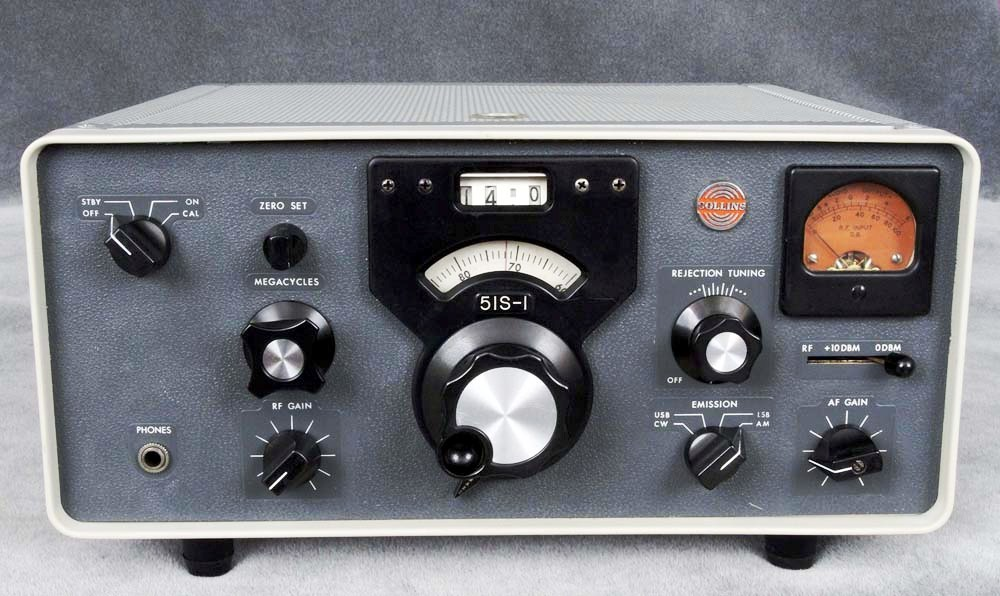
\includegraphics[scale=0.2]{Geraetetechnik/Bilder/Collins_51S-1_front.jpg}
 \vspace{-6cm}
\end{wrapfigure}

\section*{Theorie- und Prüfungsfragen} 

\mucho{1}{TB707}
{ Die Leistung eines gleichmäßig über einen Frequenzbereich verteilten Rauschens ist}%Frage
{umgekehrt proportional zur Empfängerempfindlichkeit.}%A
{proportional zum Signal-Rauschabstand.}%B
{proportional zur Bandbreite.}%C
{umgekehrt proportional zum Eingangswiderstand.}%D
{C}%Lösung

\mucho{2}{TB708}
{Wie verhält sich der Pegel des thermischen Rauschens am Empfängerausgang, wenn von einem Quarzfilter mit einer Bandbreite von 2,5 kHz auf ein Quarzfilter mit einer Bandbreite von 0,5 kHz mit gleicher Durchlassdämpfung und Flankensteilheit umgeschaltet wird? Der Rauschpegel}%Frage
{erhöht sich um etwa 7 dB.}%A
{verringert sich um etwa 20 dB.}%B
{verringert sich um etwa 7 dB.}%C
{erhöht sich um etwa 20 dB.}%D
{C}%Lösung

\mucho{3}{TF440}
{Was bedeutet Signal-Rauschabstand (S/N) bei einem VHF-Empfänger?}%Frage
{Er gibt an, um wie viel dB das Rauschsignal stärker ist als das Nutzsignal.}%A
{Er gibt an, wieviel dB stärker das Nutzsignal zum Rauschsignal ist.}%B
{Es ist der Abstand in Kilohertz zwischen Empfangssignal und Störsignal.}%C
{Es ist der Abstand in Kilohertz zwischen Empfangsfrequenz und Spiegelfrequenz.}%D
{B}%Lösung

\mucho{4}{TF441}
{Was bedeutet die Rauschzahl F=2 bei einem UHF-Vorverstärker? Das Ausgangssignal des Verstärkers hat ein}%Frage
{um 6 dB geringeres Signal-Rauschverhältnis als das Eingangssignal.}%A
{um 3 dB höheres Signal-Rauschverhältnis als das Eingangssignal.}%B
{um 3 dB geringeres Signal-Rauschverhältnis als das Eingangssignal.}%C
{um 6 dB höheres Signal-Rauschverhältnis als das Eingangssignal.}%D
{C}%Lösung

\mucho{5}{TF214}
{An welcher Stelle einer Amateurfunkanlage sollte ein VHF-Vorverstärker eingefügt werden?}%Frage
{Möglichst unmittelbar vor dem Empfängereingang}%A
{Möglichst direkt an der Antenne.}%B
{Zwischen Senderausgang und Antennenkabel}%C
{Zwischen Stehwellenmessgerät und Empfängereingang}%D
{B}%Lösung

\mucho{6}{TF410}
{Das Bild zeigt \ref{Durchlasskurve} die Durchlasskurve eines Empfängerfilters.  Es ist besonders für den Empfang von}%Frage
{CW-Signalen geeignet.}%A
{SSB-Signalen geeignet.}%B
{Breitbandfernsehsignalen geeignet.}%C
{breitbandigen FM-Signalen geeignet.}%D
{B}%Lösung

\mucho{7}{TF411}
{Das Bild zeigt \ref{Durchlasskurve} die Durchlasskurve eines Empfängerfilters.  In dem dargestellten Diagramm beträgt die Grenzbandbreite bei -60 dB etwa}%Frage
{4kHz}%A
{5,6 kHz}%B
{6 kHz}%C
{2,5kHz}%D
{A}%Lösung

\begin{figure}[H]
	\centering
	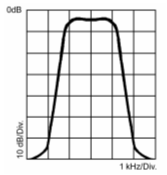
\includegraphics[scale=0.9]{Geraetetechnik/Bilder/TF410.png}
	\caption{Durchlasskurve eines Empfängerfilters}
	\label{Durchlasskurve}
	\end{figure}


\mucho{8}{TF302}
{Welche Signale steuern gewöhnlich die Empfängerstummschaltung (Squelch)?}%Frage
{Es ist das HF-Signal der Eingangsstufe.}%A
{Die ZF- oder NF-Signale.}%B
{Es ist das HF-Signal des VFO.}%C
{Es ist das ZF-Signal des BFO.}%D
{B}%Lösung

\mucho{9}{TF303}
{Was bewirkt die AGC (automatic gain control) bei einem starken Eingangssignal? Sie reduziert die}%Frage
{Es ist das HF-Signal der Eingangsstufe.}%A
{Amplitude des VFO.}%B
{Amplitude des BFO.}%C
{Höhe der Versorgungsspannungen.}%D
{A}%Lösung

\mucho{10}{TF320}
{Welche Baugruppe könnte in einem Empfänger gegebenenfalls dazu verwendet werden, um einen schmalen Frequenzbereich zu unterdrücken, in dem Störungen empfangen werden?}%Frage
{Notchfilter}%A
{Dämpfungsglied}%B
{Hochpass}%C
{Sperrfilter}%D
{A}%Lösung

